\chapter{Graphic User Interface}
\label{c:gui}

%-----------------------------------------------------------------
\section{GUI Installation}
\label{s:gui.install}

There are a number of python modules needed for the GUI:
\begin{example}
  tkinter
  ttk (may be called pyttk)
  pexpect         # If using pexpect instead of ctypes.
  matplotlib, cycler, dateutil, tkagg
\end{example}
Note: The GUI uses the TkAgg backend for matplotlib. There may be a problem with Python finding the
TkAgg backend. On the mac, using macports, the solution is to install matplotlib with the
\vn{tkinter} variant. Something like:
\begin{example}
  sudo port uninstall py36-matplotlib           # May not be needed.
  sudo port install  py36-matplotlib +tkinter   # This is when using Python version 3.6
\end{example}
For more information see:
\begin{example}
  https://matplotlib.org/tutorials/introductory/usage.html#backends
\end{example}

If one of the modules is missing, python will generate an error message. For example:
\begin{example}
> python ../../gui/main.py
Exception in Tkinter callback
Traceback (most recent call last):
  File "/opt/local/Library/Frameworks/Python.framework/Versions/3.7/lib/python3.7/tkinter/__init__.py", line 1705, in __call__
    return self.func(*args)
  File "../../gui/main.py", line 372, in param_load
    from tao_interface import tao_interface
  File "/Users/dcs16/Bmad/bmad_dist/tao/gui/tao_interface.py", line 4, in <module>
    from tao_pipe import tao_io
  File "/Users/dcs16/Bmad/bmad_dist/tao/python/tao_pexpect/tao_pipe.py", line 14, in <module>
    import pexpect
ModuleNotFoundError: No module named 'pexpect'
\end{example}
Notice that the last line shows that the pexpect module is needed.

How to install missing modules on the mac: [Note: The exact installation commands will depend upon
which version of python is being used. Use the "python --version" command to see what version you
are using.

Using macports and python 3.6:
\begin{example}
  sudo port install py36-tkinter
  sudo port install py36-pexpect
\end{example}

Using pip (or pip3):
\begin{example}
  sudo pip install pytkk
  sudo pip install pexpect
\end{example}

WARNING: it can be dangerous to use pip to install/modify modules in your system python.
A much safer way to install the modules you need is to set up a python virtual environment.
On Linux, you may also be able to find versions of the required modules in your system package manager,
which are tailored to your Linux distribution and will not break your system python.

%-----------------------------------------------------------------
\subsection{Installation Troubleshooting}
\label{s:gui.trouble}

Got error:
\begin{example}
  ImportError: cannot import name ‘_tkagg'
\end{example}

Solution: Uninstall and then reinstall matplotlib. For example, if using pip:
\begin{example}
  sudo pip uninstall matplotlib
  sudo pip install matplotlib
\end{example}

%-----------------------------------------------------------------
\subsection{Developer Setup}
\label{s:gui.develop}

For GUI development, it may be desireable to specify a local build tree as the place for the python
scripts to find the \tao executable and other modules. To accomplish this, set the environmental
variable ACC_LOCAL_ROOT to the base directory of your local build tree.


%-----------------------------------------------------------------
\section{Starting the GUI}
\label{s:gui.startup}
From your system shell, you can execute the gui with the command
\begin{example}
  python -m pytao.gui
\end{example}
either from the \texttt{tao/python} directory, or from anywhere on your system if the pytao package is installed somewhere in your python path.  You can also specify any of the command line options that tao supports.  For example,
\begin{example}
  python -m pytao.gui -init_file ~/bmad_dist/tao/examples/cesr/tao.init -rf_on
\end{example}
This will prefill the settings for \texttt{init_file} and \texttt{rf_on}.
The GUI starts with the window shown in Figure \ref{fig:startup}.
From here, all of the command-line settings that Tao supports can be set (settings that are left blank are omitted when Tao is started).

Towards the bottom of the window are some settings that are specific to the GUI.  The "Interface to Tao" setting controls whether the ctypes or pexpect backend for communicating with Tao will be used.
Below it, the "Shared Library" or "Tao executable" setting points the GUI to the correct executable or shared object library to use.
In most cases, the GUI will prefill this box by referencing the ACC_LOCAL_ROOT and ACC_ROOT_DIR environmental variables.

Finally, the font size can be set as desired.
Hitting Enter/Return while the font size box is in focus will adjust the font size of the startup window to give the user a sense of what the chosen font size will look like.

Once all of the startup settings have been set, clicking "Start Tao" will initialize Tao and bring the user to the main GUI window.
\begin{figure}
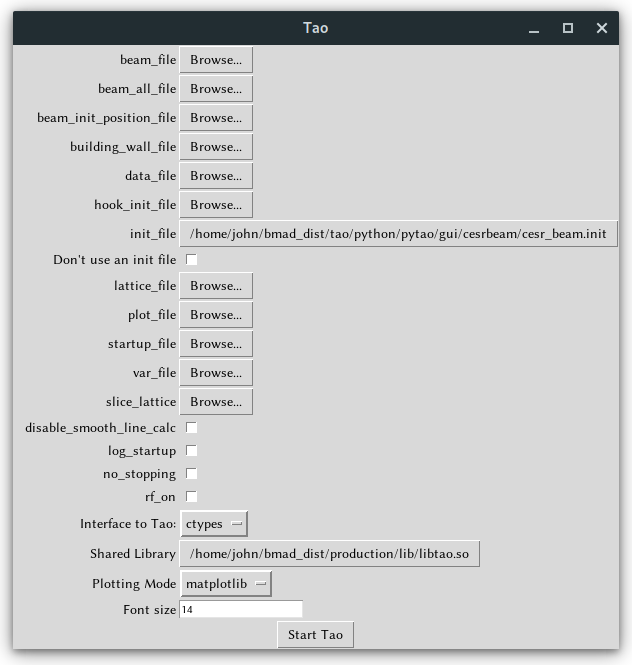
\includegraphics[width=8cm]{figures/startup.png}
\centering
\caption{The GUI startup window.  In this example, the init file that tao should use has been specified.}
\label{fig:startup}
\end{figure}

%--------------------------------------------------------------

\subsection{GUI Initialization File}
\label{s:gui.init.file}

To speed up the initialization process, you can make an init file for the GUI.  This file should be called "gui.init", and it should be in the same directory from which you initialize the GUI.

gui.init should have each option on a separate line, and each option should be listed in the form "parameter:value".  For example, the text below would constitute a good gui.init file:

\begin{example}
  #MY GUI INIT FILE
  beam_file:/path/to/beam/file
  data_file:/path/to/data/file
  #THIS IS A COMMENT
  disable_smooth_line_calc:T
  rf_on:T
  tao_exe:/path/to/executable
\end{example}

The order in which you list options in gui.init is not important.

File paths should be specified in full to be safe, but you can specify paths relative to the directory from which you launch main.py.  For example, "/home/username/file", "subfolder/my_file", and "../../path/to/another/file" would all be acceptable file paths.  You can also use your environmental variables and "\textasciitilde{}", as in "\textasciitilde{}/Documents/my_file" and "\$DIST_BASE_DIR/tao/file".

Logic (true/false) options may be specified by T/F or True/False.

You can also include comments with \#.  Any line with \# as its first non-whitespace character will be considered a comment and ignored.

%-----------------------------------------------------------------

\section{The Main GUI Window}
\label{s:gui.root.window}

The main window for the GUI is shown in Figure \ref{fig:root.window}.
\begin{figure}
\centering
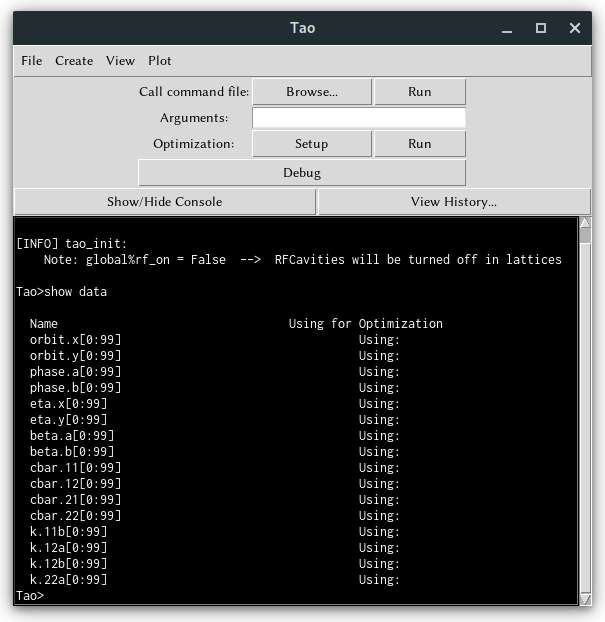
\includegraphics[width=8cm]{figures/root_window.png}
\caption{The main GUI window, showing the results of \texttt{show data} on the console.}
\label{fig:root.window}
\end{figure}
From here, the user has access to all of the GUI's features.
Command files can be called by browsing for them and then clicking "Run", with arguments specified in the "Arguments" below.
In the future, the user will also be able to set up and run optimization routines from this window, although this feature is not currently available.

The main window also has a console, where commands can be run in Tao exactly like in regular Tao.
The console will also display warning messages if a command produces an error.

%-----------------------------------------------------------------

\section{Global Variables}
\label{s:gui.global.variables}

Global variables in Tao can be viewed and modified from the global variables window as shown in Figure \ref{fig:gui.global.variables}.
Once you have editted the global variables, clicking the "Set Global Variables" button will set the variables in Tao as appropriate.

\begin{figure}
\centering
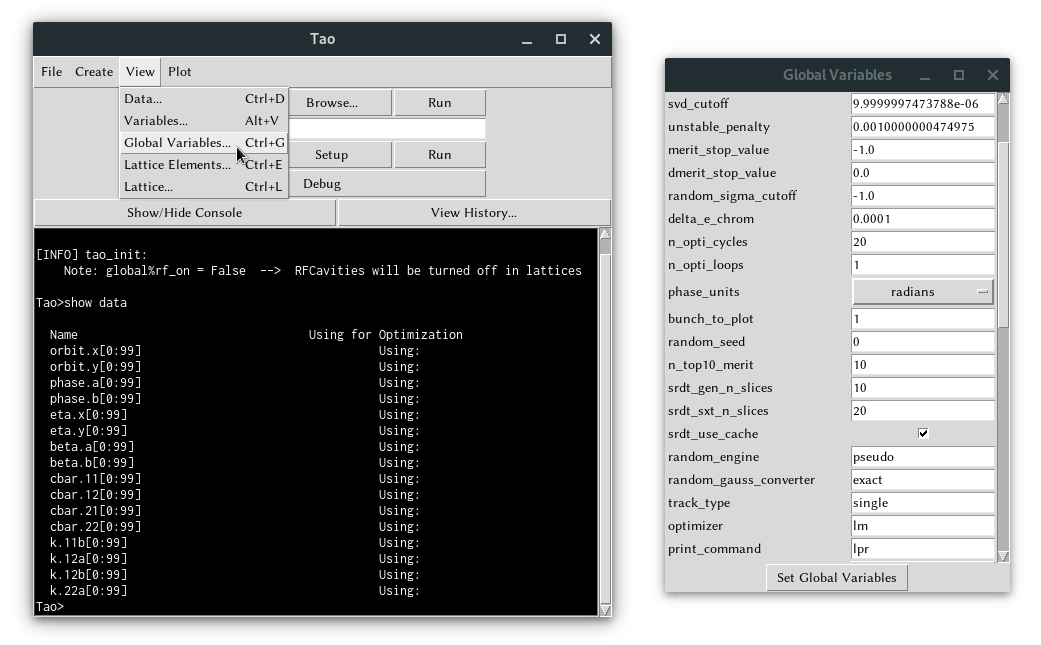
\includegraphics[width=10cm]{figures/globals.png}
\caption{View and edit global variables with the Global Variables window.}
\label{fig:gui.global.variables}
\end{figure}

%-----------------------------------------------------------------
\section{Data}
\label{s:gui.data}

The GUI provides several windows for viewing and editing data arrays.

\subsection{Viewing Data}
\label{s:gui.data.view}

Figure \ref{fig:gui.data.view} shows the various windows that the GUI provides for viewing data and making minor changes to data arrays.
\begin{figure}
\centering
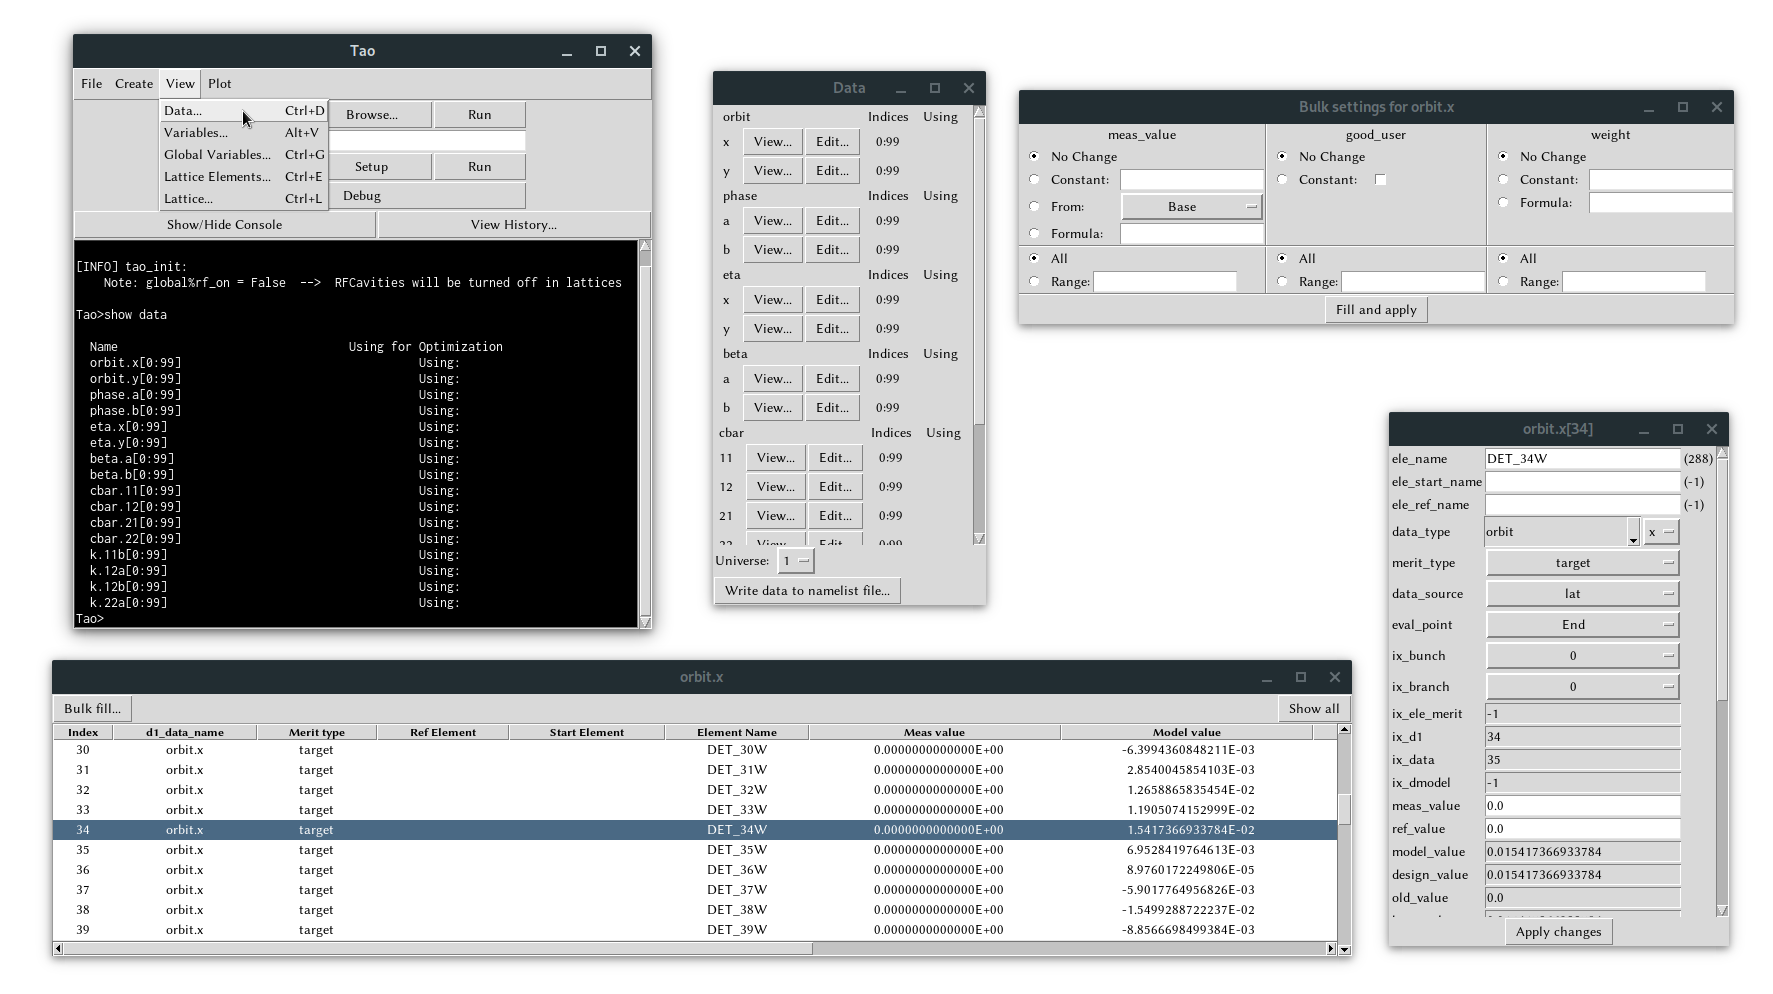
\includegraphics[width=12cm]{figures/view_data.png}
\caption{The GUI's data viewing windows.
Top left: the Tao root window and the menu shortcut for viewing data.
Top middle: The d2_data_array window, which list the currently defined d2_data_arrays for each universe.
This window also includes links to view and edit (see section \ref{s:gui.data.edit}) existing d1_data_arrays.
Bottom left: The d1_data_array window (in this case for orbit.x), showing all of the datums in the array orbit.x.
Bottom right: The individual datum window (in this case for orbit.x[34]) displaying detailed datum properties and allowing the user to edit some of these properties.
Top right: The bulk edit window (in this case for orbit.x) providing controls to quickly edit a few key properties for multiple datums in a d1_data_array.}
\label{fig:gui.data.view}
\end{figure}

The d2_data_array window (top middle in Figure \ref{fig:gui.data.view}) displays all data arrays for a given universe.
To view any existing d1_data_array, click on its "View" button.
This window also provides the ability to edit any existing data array in detail (see Section \ref{s:gui.data.edit}), as well as functionality for writing existing data to a namelist (see Section \ref{s:gui.namelist}).

The d1_data_array window (bottom left in Figure \ref{fig:gui.data.view}) allows the user to view an existing d1_data_array.
This window displays important properties of each datum in the array, such as element name, meas, model, and design values, and weight, in a scrollable table.
To view a datum in detail, double click on its row in the d1_data_array window.
This will open the individual datum window for that datum, displaying all of its properties and allowing some of them to be editted.

The d1_data_array window also allows the user to edit a few key properties of the datums in the array all at once using the bulk settings window (top right in Figure \ref{fig:gui.data.view}).
This window is accessed by clicking on the "Bulk fill" button in the d1_data_array window.
From here, the meas_value, good_user, and weight settings for the datums in the array can be edited in bulk.
Changes may be applied to every datum in the array, or to only a specific range of datums using the range specifier.
Once the desired settings have been specified, clicking the "Fill and apply" button will edit the d1_data_array as necessary, and changes will be reflected in the d1_data_array window.

\subsection{Creating and Editing Data}
\label{s:gui.data.edit}

%-----------------------------------------------------------------
\section{Plotting}
\label{s:gui.plot}

Interacting with plots in the GUI is primarily done using the toolbar along the bottom of the plotting window.

Starting from the left, the home button returns the graph to the starting view. The back button returns to the previous view of the graph, working as an undo button. The forward button undoes the effects of the back button. All of these buttons also have keyboard shortcuts, 'h' or 'r' for home, 'c' or 'left arrow' for back, and 'v' or 'right arrow' for forward.

The pan/zoom button allows panning of the graph by holding a left click on the graph and dragging the mouse around. his mode also allows zooming of the graph by holding a right click on the graph and dragging the mouse around. These actions can be restricted to the horizontal axis by holding 'x' while dragging, or the vertical axis by holding 'y'. Holding 'control' while dragging the mouse will preserve aspect ratio. Clicking on the toolbar button again will get out of this mode.

The zoom to rectangle button allows a rectangle to be selected by holding a left click on the graph and dragging the mouse, which will then fill the graph window. Holding 'x' or 'y' while selecting a rectangle will only effect the horizontal or vertical axis respectively.

The save button allows the graph window to be saved as an image file. Using 'ctrl+s' has the same effect.

If any floor plan or lat layout is present, double clicking on an element will open a window to view or edit element parameters.

Floor plans contain a slider to scale the size of elements away from the element centerline. Clicking on the slider will adjust the width of the displayed elements.

%-----------------------------------------------------------------
\subsection{Plotting Initialization}
\label{s:gui.plot.init}

When operating the GUI in matplotlib mode, you can specify a list of template plots to plot in matplotlib as soon as tao starts.  These templates should be listed in a file called plot.gui.init, which should be in the same directory from which you launch the gui.

plot.gui.init should have one template listed per line and absolutely nothing else on the line.  The templates listed in plot.gui.init are checked against the list of templates that tao can plot, and if a template is not recognized it is simply ignored.


%-----------------------------------------------------------------
\section{Lattice Templates}
\label{s:gui.lat}

You can save your settings from the lattice table window in a template file, which can then be loaded and added to from within the gui.
The file can be named anything, and the formatting is as follows:
Lines starting with \# are considered comments and ignored.
Lines starting with "name:" are interpreted as a name for the settings listed in the line directly below
All other lines are interpreted as switches, as would be used with the show lattice command in Tao (see the tao manual for more info).
All switches for a given template should be on one line.

Example:
\begin{example}
#MY TEMPLATE FILE
name:template 1
-orbit -spin -tracking_elements
name:template 2
-lords q*
name: another template
-floor_coords -s 10:20
-radiation_integrals -all
\end{example}

This template file defines four templates: "template 1", "template 2", "another template", and an unnamed template (which has the switches -radiation_integrals -all).  Named templates are displayed by name in the gui, while unnamed templates are simply displayed by what switches they specify.

%-----------------------------------------------------------------
\section{Writing Namelists}
\label{s:gui.namelist}
